\documentclass{beamer}

\usepackage{amsmath}
\usepackage[style=alphabetic,url=true]{biblatex}
\usepackage{environ}
\usepackage{geometry}
\usepackage{graphicx}
\usepackage{amsmath}
\usepackage{amsfonts}
\usepackage{amssymb}
\usepackage{calrsfs}
\usepackage{listings}
\usepackage{tikz}
\usepackage[T2A]{fontenc}
\usepackage[utf8]{inputenc}
\usepackage[cache=false]{minted}

\graphicspath{ {./graphics/} }
\usetikzlibrary{shapes.arrows,chains}
\usecolortheme{beaver}
\setbeamertemplate{itemize item}[circle]
\setbeamertemplate{itemize subitem}{--}
\addtobeamertemplate{navigation symbols}{}{
  \usebeamerfont{footline}
  \usebeamercolor[fg]{footline}
  \hspace{1em}
  \insertframenumber/\inserttotalframenumber
}
\setminted[Lisp]{
  fontsize=\scriptsize
}
\setminted[text]{
  fontsize=\tiny
}
\usemintedstyle{xcode}
\BeforeBeginEnvironment{minted}{\medskip}
\AfterEndEnvironment{minted}{\medskip}



\title{
  Common Lisp and Introduction to Functional Programming \\
  Lecture 9: Functional Data Structures 2/2
}
\author{Yuri Zhykin}
\date{Apr 14, 2021}

\begin{document}

\frame{\titlepage}

\begin{frame}[fragile]
  \frametitle{Functional Data Structures}
  \begin{itemize}
  \item \textbf{Persistent} data structures are data structures that allow
    \textbf{multiple versions} of the data structure to exist at the same time.
  \item \textbf{Ephemeral} data structures are data structures that allow only a
    \textbf{single version} to exist at a time.
  \item In functional programming languages \textbf{all} data structures are
    persistent.
  \end{itemize}
\end{frame}

\begin{frame}[fragile]
  \frametitle{Structure Sharing}
  \begin{itemize}
  \item Every operation that \textbf{updates} a persistent data structures,
    \textbf{creates a new version} of the data structure with the contents that
    correspond to the updated data.
  \item \textbf{Persistent} data structures are inefficient when fully copied.
  \item Efficiency can be achieved by utilizing \textbf{structure sharing}.
  \item Common Lisp's list is a persistent data structure.
  \item More complex structure-sharing data structures can be built on lists.
  \end{itemize}
\end{frame}

\begin{frame}[fragile]
  \frametitle{Stacks 1/2}
  \begin{itemize}
  \item \textbf{Stack} is an a collection of elements with two operations:
    \begin{itemize}
    \item \textbf{push} - add an element to the collection,
    \item \textbf{pop} - remove \textbf{the most recently added element} from
      the collection (\textbf{LIFO}, \textbf{Last In, First Out}).
    \end{itemize}
  \item Common Lisp has built-in \textbf{destructive} operations
    \mintinline{Lisp}{push} and \mintinline{Lisp}{pop} for using lists as
    stacks:
\begin{minted}{Lisp}
  CL-USER> (setq s '(1 2 3))
  (1 2 3)
  CL-USER> (push 0 s)
  (0 1 2 3)
  CL-USER> (pop s)
  0
  CL-USER> s
  (1 2 3)
\end{minted}
  \end{itemize}
\end{frame}

\begin{frame}[fragile]
  \frametitle{Stacks 2/2}
  \begin{itemize}
  \item Functional stack can be trivially implemented as follows:
\begin{minted}{Lisp}
  ;; Simply construct a new list with a new element at its head.
  (defun stack-push (e s)
    (cons e s))

  ;; Return both the top stack value and the new version of stack.
  (defun stack-pop (s)
    (values (car s) (cdr s)))
\end{minted}
  \item Example:
\begin{minted}{Lisp}
  CL-USER> (let ((s0 nil))
             (format t "s0: ~a~%" s0)
             (let ((s1 (stack-push 1337 s0)))
               (format t "s1: ~a~%" s1)
               (multiple-value-bind (v s2) (stack-pop s1)
                 (format t "s2: ~a~% v: ~a~%" s2 v))))
  s0: nil
  s1: (1337)
  s2: nil
   v: 1337
\end{minted}    
  \end{itemize}
\end{frame}

\begin{frame}[fragile]
  \frametitle{Dictionaries}
  \begin{itemize}
  \item \textbf{Dictionary} or \textbf{finite map} is a collections of key-value
    associations:
    \begin{itemize}
    \item \textbf{insert} - add a key-value association,
    \item \textbf{delete} - remove an association between a key and its value,
    \item \textbf{lookup} - find an associated value for a given key.
    \end{itemize}
  \item Dictionaries can be represented with lists (e.g. built-in \textbf{plist}
    and \textbf{alist} structures).
  \item Sequential representation is inefficient:
    \begin{itemize}
    \item \textbf{insert} is $O(1)$, but
    \item \textbf{delete} is $O(n)$ and
    \item \textbf{lookup} is $O(n)$ as well.
    \end{itemize}
  \end{itemize}
\end{frame}

\begin{frame}[fragile]
  \frametitle{Trees}
  \begin{itemize}
  \item \textbf{Structure-sharing dictionary} can be implemented with the
    \textbf{tree} data structure.
  \item Example: operation that inserts new node $e$, must created new nodes
    $d'$, $g'$ and $f'$, but can share nodes $b$ and all its children.
  \end{itemize}
  \begin{center}
    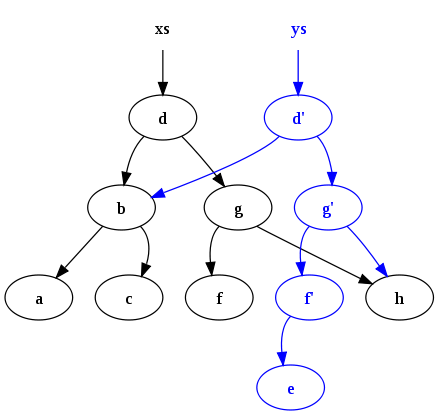
\includegraphics[width=0.6\textwidth]{bst.png}
  \end{center}
\end{frame}

\begin{frame}[fragile]
  \frametitle{Binary Search Trees 1/5}
  \begin{itemize}
  \item \textbf{Binary search tree} (\textbf{BST}) is a \textbf{rooted}
    \textbf{binary tree} whose internal nodes each store a key
    \begin{itemize}
    \item each node contains a \textbf{key} and, \textit{optionally}, an
      associated \textbf{value},
    \item each node has two subtrees (children), denoted \textbf{left} and
      \textbf{right},
    \item \textbf{binary search property}: for every node its key is greater
      than all the keys in the node's left subtree and less than those in its
      right subtree.
    \end{itemize}
  \item \textit{On average}, binary tree allows for significantly more efficient
    operations (still $O(n)$ in the worst case):
    \begin{itemize}
    \item \textbf{insert} is $O(\log{n})$,
    \item \textbf{delete} is $O(\log{n})$,
    \item \textbf{lookup} is $O(\log{n})$.
    \end{itemize}
  \end{itemize}
\end{frame}

\begin{frame}[fragile]
  \frametitle{Binary Search Trees 2/5}
  \begin{itemize}
  \item Binary search trees can be built on top of lists using the following
    \textbf{abstraction}:
\begin{minted}{Lisp}
  (defun make-tree ()
    nil)

  (defun make-node (key value left right)
    (list key value left right))

  (defun node-key (node)
    (first node))

  (defun node-value (node)
    (second node))

  (defun node-left-child (node)
    (third node))

  (defun node-right-child (node)
    (fourth node))
\end{minted}    
  \end{itemize}
\end{frame}

\begin{frame}[fragile]
  \frametitle{Binary Search Trees 3/5}
  \begin{itemize}
  \item \textbf{Insert} operation works as follows:
\begin{minted}{Lisp}
(defun tree-insert (node key value)
  (cond ((null node)
         (make-node key value nil nil))
        ((string= key (node-key node))
         (make-node key
                    value
                    (node-left-child node)
                    (node-right-child node)))
        ((string< key (node-key node))
         (make-node (node-key node)
                    (node-value node)
                    (tree-insert (node-left-child node) key value)
                    (node-right-child node)))
        (t ;; (string> key (node-key node))
         (make-node (node-key node)
                    (node-value node)
                    (node-left-child node)
                    (tree-insert (node-right-child node) key value)))))
\end{minted}    
  \end{itemize}
\end{frame}

\begin{frame}[fragile]
  \frametitle{Binary Search Trees 4/5}
  \begin{itemize}
  \item \textbf{Lookup} operation is straightforward:
\begin{minted}{Lisp}
(defun tree-lookup (node key)
  (cond ((null node)
         (values nil nil))
        ((string= key (node-key node))
         (values (node-value node) t))
        ((string< key (node-key node))
         (tree-lookup (node-left-child node) key))
        (t ;; (string> key (node-key node))
         (tree-lookup (node-right-child node) key))))
\end{minted}    
  \end{itemize}
\end{frame}

\begin{frame}[fragile]
  \frametitle{Binary Search Trees 5/5}
  \begin{itemize}
  \item \textbf{Delete} operation is slightly more complicated because the
    \textbf{binary search property} must be preserved, so the tree must be
    rebalanced.
  \item If the values being inserted are \textbf{ordered}, the tree becomes
    \textbf{degenerate} and will provide worst case $O(n)$ performance.
  \item Self-balancing structures like \textbf{red-black trees} can be used to
    mitigate that.
  \end{itemize}
\end{frame}

\begin{frame}[fragile]
  \frametitle{Queues 1/5}
  \begin{itemize}
  \item \textbf{Queue} is a collection of entities that can be modified by the
    addition of entities at one end of the sequence and the removal of entities
    from the other end of the sequence.
  \item By convention, the end of the sequence where elements are added is
    called the \textbf{back} or \textbf{tail} of the queue.
  \item The end where elements are removed is called the \textbf{front} or
    \textbf{head} of the queue.
  \item Queue data structure has two main operations:
    \begin{itemize}
    \item \textbf{enqueue} - add an element to the queue,
    \item \textbf{dequeue} - take an element from the queue in the \textbf{FIFO}
      (\textbf{First In, First Out}) order.
    \end{itemize}
  \end{itemize}
\end{frame}

\begin{frame}[fragile]
  \frametitle{Queues 2/5}
  \begin{itemize}
  \item Using list as a queue is inefficient, because only one operation can be
    implemented efficiently:
    \begin{itemize}
    \item \textbf{enqueue} is $O(1)$, then \textbf{dequeue} $O(n)$ or
    \item \textbf{dequeue} is $O(1)$, then \textbf{enqueue} $O(n)$.
    \end{itemize}
  \item Efficient queue can be constructed by splitting the queue list into two
    parts:
    \begin{itemize}
    \item first part, \textbf{front}, is sorted \textbf{from the least recent to
        the most recent element},
    \item second part, \textbf{back}, is sorted \textbf{from the most recent to
        the least recent element},
    \item \textbf{enqueue} operation adds a new element to the \textbf{head} of
      the \textbf{front} list,
    \item \textbf{dequeue} operation takes the \textbf{head} of the
      \textbf{back} list as the result.
    \end{itemize}
  \end{itemize}
\end{frame}

\begin{frame}[fragile]
  \frametitle{Queues 3/5}
  \begin{itemize}
  \item The following queue
    $$Q = (1, 2, 3, 4, 5)$$
    is represented internally like this
\begin{minted}{text}
          +---+   +---+   +---+   +---+            
   front: | 1 |-->| 2 |-->| 3 |-->|NIL|            
          +---+   +---+   +---+   +---+
          +---+   +---+   +---+            
   back:  | 5 |-->| 4 |-->|NIL|            
          +---+   +---+   +---+            
\end{minted}
  \item Adding an element $6$ to the queue results in
\begin{minted}{text}
          +---+   +---+   +---+   +---+            
   front: | 1 |-->| 2 |-->| 3 |-->|NIL|            
          +---+   +---+   +---+   +---+
          +---+   +---+   +---+   +---+            
   back:  | 6 |-->| 5 |-->| 4 |-->|NIL|            
          +---+   +---+   +---+   +---+            
\end{minted}
  \item Taking an element from the queue results in
\begin{minted}{text}
          +---+   +---+   +---+            
   front: | 2 |-->| 3 |-->|NIL|            
          +---+   +---+   +---+
          +---+   +---+   +---+   +---+            
   back:  | 6 |-->| 5 |-->| 4 |-->|NIL|            
          +---+   +---+   +---+   +---+            
\end{minted}
  \end{itemize}
\end{frame}

\begin{frame}[fragile]
  \frametitle{Queues 4/5}
  \begin{itemize}
  \item If the \textbf{front} of the queue is empty, but the \textbf{back} is
    not, we need to move the element from the \textbf{back} to the
    \textbf{front}:
    \begin{itemize}
    \item before
\begin{minted}{text}
          +---+            
   front: |NIL|            
          +---+
          +---+   +---+   +---+   +---+            
   back:  | 6 |-->| 5 |-->| 4 |-->|NIL|            
          +---+   +---+   +---+   +---+            
\end{minted}
    \item after
\begin{minted}{text}
          +---+   +---+   +---+   +---+            
   front: | 4 |-->| 5 |-->| 6 |-->|NIL|            
          +---+   +---+   +---+   +---+            
          +---+            
   back:  |NIL|            
          +---+
\end{minted}
    \end{itemize}
  \end{itemize}
\end{frame}

\begin{frame}[fragile]
  \frametitle{Queues 5/5}
  \begin{itemize}
  \item The queue implementation above satisfies the requirement
    \begin{itemize}
    \item \textbf{enqueue} runs in $O(1)$,
    \item \textbf{dequeue} runs in $O(1)$, $O(n)$ in the worst case.
    \end{itemize}
  \item The operation of moving the elements from the \textbf{back} to the
    \textbf{front} causes the worst case scenario for \textbf{dequeue}
    operation, but it only happens when the \textbf{front} is empty.
  \item The $O(n)$ cost of moving the element from the \textbf{back} to the
    \textbf{front} is \textbf{amortized} across multiple $O(1)$ operations.
  \end{itemize}
\end{frame}

\begin{frame}[fragile]
  \frametitle{Amortized Analysis 1/2}
  \begin{itemize}
  \item \textbf{Amortized analysis} is an approach to complexity analysis that
    considers the possible sequences of operations instead of isolated
    operations.
  \item First formally introduced by Robert Tarjan in his 1985 paper
    \textit{Amortized Computational Complexity}.
  \item The basic idea is that a \textbf{worst-case operation} can alter the
    state in such a way that the \textbf{worst case cannot occur again for a
      long time}, thus ``amortizing'' its cost.
  \end{itemize}
\end{frame}

\begin{frame}[fragile]
  \frametitle{Amortized Analysis 2/2}
  \begin{itemize}
  \item Three main ways to perform amortized analysis:
    \begin{itemize}
    \item the \textbf{aggregate method} (determine the upper bound $T(n)$ on the
      total cost of a sequence of $n$ operations, then calculate the amortized
      cost to be $T(n) / n$),
    \item the \textbf{accounting method}, (operations have a cost higher than
      the actual cost, accumulating a saved ``credit'' that is used to ``pay''
      for the later operations),
    \item the \textbf{potential method} (operation has a cost and a change in
      potential, which is some function of the state of the data structure).
    \end{itemize}
  \end{itemize}
\end{frame}

\begin{frame}[fragile]
  \frametitle{Useful Resources}
  \begin{minipage}{0.6\textwidth}\raggedright
    \begin{itemize}
    \item \textbf{Purely Functional Data Structures} by Chris Okasaki
    \end{itemize}
  \end{minipage}
  \begin{minipage}{0.3\textwidth}
    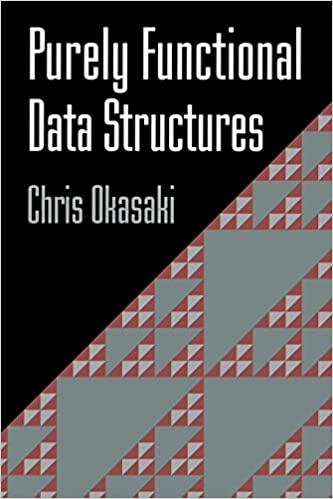
\includegraphics[width=\linewidth]{pfds}
  \end{minipage}
\end{frame}

\begin{frame}
  \frametitle{The End}
  \begin{center}
    Thank you!
  \end{center}
\end{frame}

\end{document}

%%% Local Variables:
%%% mode: latex
%%% TeX-master: t
%%% TeX-command-extra-options: "-shell-escape"
%%% End:
